\documentclass{SPC}

% IEIE Transactions on Smart Processing and Computing submission manuscript.
% SPC.cls is retained byte-for-byte; the review-copy overrides below correct
% its legacy short page and suppress editorial metadata that authors cannot set.
\usepackage{url}
\usepackage{array,tabularx}
\usepackage{multicol}
\usepackage{multirow}
\usepackage{subfigure}
\usepackage{microtype}
\usepackage{iftex}
\ifXeTeX
  \usepackage{fontspec}
  \defaultfontfeatures{Ligatures=TeX}
  \setmainfont{Times New Roman}
  \setsansfont{Arial}
  \setmonofont{Menlo}
  % SPC.cls saves \hbar through a legacy math-font hook; fontspec resets that
  % saved command.  Restore the saved definition before begin-document hooks.
  \makeatletter
  \def\s@vedhbar{\mathchar'26\mkern-9mu h}
  \makeatother
\fi

% The supplied legacy class emits an approximately 210 x 280 mm page.
% Current IEIE SPC instructions require 210 x 297 mm (A4).
\setlength{\paperwidth}{210mm}
\setlength{\paperheight}{297mm}
\special{papersize=210mm,297mm}

% Volume, issue, DOI, dates, and copyright are assigned by the journal.
\journalvolume{}
\journalnumber{}
\journalyear{}
\journalmonth{}
\setarticlestartpagenumber{1}

\allowdisplaybreaks
\newcommand{\mf}{Macro-F1}
\newcommand{\fullft}{Full FT}

% Neutral review-copy running matter.  This prevents SPC.cls from printing its
% obsolete JSTS DOI prefix, placeholder issue data, and 2024 copyright.
\makeatletter
\ifXeTeX
  % Use the configured Arial family in the title block instead of the class's
  % legacy PostScript Helvetica family switch.
  \patchcmd{\@maketitle}{\renewcommand{\rmdefault}{phv}}{\sffamily}{}{}
\fi
% Editorial dates are assigned after peer review.  The legacy class always
% prints a date row, so suppress both of its variants in the review copy.
\patchcmd{\@maketitle}{Received: \@received; Accepted: \@accepted; Published: \@published}{}{}{}
\patchcmd{\@maketitle}{Received:\@received; Revised: \@revised; Accepted: \@accepted; Published: \@published}{}{}{}
\renewcommand{\runningtitle}[2]{%
  \pagestyle{fancy}%
  \fancyhf{}%
  \fancyhead[LO]{\it\fontsize{8pt}{10pt}\selectfont IEIE Transactions on Smart Processing and Computing --- Manuscript under review}%
  \fancyhead[RO]{\fontsize{8pt}{10pt}\selectfont\thepage}%
  \fancyhead[LE]{\textbf{\thepage}}%
  \fancyhead[RE]{\fontsize{8pt}{9pt}\selectfont\it #1: #2}%
  \renewcommand{\headrulewidth}{0pt}%
  \renewcommand{\footrulewidth}{0pt}%
  \fancypagestyle{plain}{%
    \fancyhf{}%
    \fancyhead[L]{\begin{flushleft}\it\fontsize{9pt}{10pt}\selectfont\textbf{IEIE Transactions on Smart Processing and Computing}\\[-1pt]\rm\fontsize{8pt}{9pt}\selectfont Manuscript submitted for peer review\end{flushleft}}%
    \fancyhead[R]{\begin{flushright}\bf\thepage\end{flushright}}%
    \renewcommand{\headrulewidth}{0pt}%
    \renewcommand{\footrulewidth}{0pt}%
  }%
  \thispagestyle{plain}%
}
\renewcommand{\endofpaper}{%
  \vfill\noindent\rule{\linewidth}{0.3pt}%
}
\makeatother

\begin{document}

\title{Performance, Efficiency, and Collapse-Aware Stability Trade-offs in Parameter-Efficient Fine-Tuning Across Domains}

\author{Yuseok Hong*, Seonyeok Lee, and Sooyong Lee}
\institute{Major in Big Data Convergence, Sangmyung University, Seoul, Republic of Korea}
\authoremails{Yuseok Hong: hyscodebase@gmail.com}
\correspondingauthor{Yuseok Hong, hyscodebase@gmail.com}

% Keep the class variables defined even though their title row is suppressed.
\received{}
\revised{}
\accepted{}
\published{}

\begin{abstract}
Choosing a fine-tuning strategy requires balancing predictive performance, wall-clock time, trainable parameters, and stability. We reintegrate an aggregate benchmark configured for 550 runs across 13 English and Korean text-classification tasks, 22 task--model conditions, five methods, and five seeds with a collapse-aware 100-run follow-up. In the fixed-policy benchmark, full fine-tuning led 19 of 22 conditions (mean Macro-F1 0.7588), BitFit was fastest in all 22, and IA3 used the fewest trainable parameters in all 22. A task-level Friedman test showed differences among method ranks, but four of 110 method rows had an exact zero Macro-F1 standard deviation and matched the analytical fingerprint of constant-class prediction. Excluding the two affected tasks preserved the global rank difference while weakening three of four Holm-adjusted pairwise conclusions. In the paired follow-up, baseline collapse occurred in 17 of 20 full-data runs; none of the 20 combined-remedy runs collapsed, and Macro-F1 increased in every same-seed comparison, with an exact two-sided sign-flip p-value of 0.0625 and a 2.32--2.56-fold time cost. No single strategy jointly optimized every criterion, and score stability was meaningful only after a non-degeneracy check.
\end{abstract}

\begin{keywords}
Parameter-efficient fine-tuning, Text classification, Macro-F1, Training efficiency, Prediction collapse, Seed stability
\end{keywords}

\maketitle

\runningtitle{Hong et al.}{Collapse-Aware PEFT Trade-offs Across Domains}


\section{Introduction}

Fine-tuning a pretrained language model for every downstream domain can deliver strong predictive performance but duplicates a complete trainable model for each task. Parameter-efficient fine-tuning (PEFT) instead updates compact modules, low-rank matrices, activation scales, or selected parameters \cite{5,6,7,8,21}. The appeal is practical, but the phrase ``parameter efficient'' does not imply that a method is simultaneously accurate, fast, compact, and robust to the random seed. Those objectives can diverge.

Repeated runs are therefore necessary. Initialization, data order, and optimization details can materially alter a fine-tuned model \cite{9,10,17,18,19}. Yet variance alone is not a sufficient notion of stability. On an imbalanced task, every seed may converge to the same constant-class predictor. Its score standard deviation (SD) is then exactly zero even though the classifier does not discriminate among classes. A variance-only ranking can reward repeated failure.

This paper integrates two stages of one study. The first is the original fixed-policy benchmark: five fine-tuning methods, five seeds, 13 unique tasks, and 22 task--model conditions configured for 550 runs. The second is a targeted 100-run follow-up prompted by four exact-zero SD rows. The broad benchmark estimates performance, training-time, parameter, and seed-sensitivity trade-offs; the follow-up audits the zero values and tests one combined recovery configuration. Remedy results are not inserted into the original ranking because only post-selected failed cells received the larger optimization budget.

We ask four research questions (RQs).

\begin{itemize}
\item \textbf{RQ1:} How do Full FT, LoRA, Adapter, IA3, and BitFit rank in predictive performance across the original tasks?
\item \textbf{RQ2:} How do wall-clock time and trainable-parameter rankings differ from performance rankings?
\item \textbf{RQ3:} Which task--model interactions create local exceptions, and how sensitive are conclusions to split and collapse concerns?
\item \textbf{RQ4:} Do the exact-zero SD rows reflect useful repeatability or degenerate prediction, and can a paired combined remedy recover them?
\end{itemize}

The contributions are: (1) restoration of the original multi-criteria benchmark and task-level inference; (2) collapse-aware reanalysis of the four exact zeros; (3) split- and collapse-sensitivity analyses that expose which conclusions are robust; (4) a 100-run pilot and full-data paired follow-up with prediction-distribution diagnostics; and (5) an auditable manuscript build that deterministically regenerates downstream statistics and figures from the preserved aggregate snapshot while keeping post-selected remedy evidence separate.


\section{Related Work}

\subsection{Fine-Tuning and Parameter Efficiency}

BERT \cite{1}, RoBERTa \cite{2}, BERTweet \cite{3}, and KLUE RoBERTa \cite{4} support comparisons across general English, social-media, and Korean text. Adapters insert trainable bottlenecks \cite{5}; LoRA factorizes a trainable weight update \cite{6}; IA3 learns activation-scaling vectors \cite{7}; and BitFit updates bias terms \cite{8}. UniPELT combines several PEFT mechanisms \cite{20}, while a broader survey shows that efficiency depends on implementation and deployment context as well as trainable parameter count \cite{21}.

One prior empirical study reported task-dependent outcomes rather than a universal PEFT winner. A three-task GLUE study by Hong and Kim \cite{23} compared full, LoRA, prompt, and selective fine-tuning. The present work does not reuse those GLUE result cells: it expands to 13 different English and Korean tasks, three pretrained checkpoints, five seeds, Adapter/IA3/BitFit, wall-clock and parameter measurements, and a run-level collapse follow-up.

\subsection{Seed Stability and Degenerate Solutions}

Score distributions reveal conclusions hidden by single runs \cite{9}. Fine-tuning instability can arise from optimization and data order, and longer or better-specified training can improve stability \cite{10,17,18}. Recent work continues to find macro- and micro-level seed effects in language-model fine-tuning \cite{19}. These studies motivate repetition but do not make a small SD intrinsically desirable.

Macro-F1 weights each class equally and is useful under imbalance, but a constant predictor receives a deterministic, nonzero value. A joint check of accuracy, macro precision, macro recall, and Macro-F1 can therefore reveal an aggregate constant-class fingerprint. Direct prediction counts are stronger evidence and are retained in our follow-up. We treat performance, time, parameter footprint, and \emph{non-degenerate} stability as separate axes rather than collapsing them into one unvalidated score.


\section{Study Design}

\subsection{Original Benchmark Scope}

The benchmark crosses Full FT, LoRA, Adapter, IA3, and BitFit with seeds 42, 52, 62, 72, and 82. Study 1 uses BERTweet on the Measuring Hate Speech corpus \cite{22,27}; Study 2 uses BERTweet and RoBERTa on nine English tasks; Study 3 uses KLUE RoBERTa on three Korean tasks. Table \ref{tab:datasets} gives the processed splits, model coverage, and epoch budget. The 22 task--model conditions yield 110 method rows and a configured design of $22\times5\times5=550$ runs. Because historical run-level files are absent, ``configured'' is used instead of claiming that all 550 executions can now be independently audited.

\begin{table*}[!t]
\caption{Original benchmark datasets and processed split sizes. We use five of TweetEval's seven tasks \cite{11}; FinancialPhraseBank \cite{12}, IMDb \cite{13}, Amazon Reviews \cite{14}, AG News \cite{15}, KLUE \cite{4}, NSMC \cite{26}, and K-MHaS \cite{16} supply the others. BTw = BERTweet; RBa = RoBERTa; K-R = KLUE RoBERTa.}
\label{tab:datasets}
\centering
\scriptsize
\setlength{\tabcolsep}{2.8pt}
\begin{tabularx}{\textwidth}{clXcrrrlc}
\toprule
Study & Task & Source & $K$ & Train & Val. & Test & Model(s) & Epochs \\
\midrule
1 & Measuring hate speech & UC Berkeley D-Lab & 2 & 108,444 & 13,556 & 13,556 & BTw & 3 \\
2 & Tweet sentiment & TweetEval sentiment & 3 & 45,615 & 2,000 & 12,284 & BTw, RBa & 2 \\
2 & Finance sentiment & FinancialPhraseBank & 3 & 3,872 & 484 & 484 & BTw, RBa & 2 \\
2 & Movie reviews & IMDb & 2 & 22,500 & 2,500 & 25,000 & BTw, RBa & 2 \\
2 & Product reviews & Amazon Reviews Multi & 5 & 200,000 & 5,000 & 5,000 & BTw, RBa & 2 \\
2 & Tweet emotion & TweetEval emotion & 4 & 3,257 & 374 & 1,421 & BTw, RBa & 2 \\
2 & Tweet hate & TweetEval hate & 2 & 9,000 & 1,000 & 2,970 & BTw, RBa & 2 \\
2 & Tweet offensive & TweetEval offensive & 2 & 11,916 & 1,324 & 860 & BTw, RBa & 2 \\
2 & Tweet irony & TweetEval irony & 2 & 2,862 & 955 & 784 & BTw, RBa & 2 \\
2 & News topic & AG News & 4 & 108,000 & 12,000 & 7,600 & BTw, RBa & 2 \\
3 & News topic & KLUE YNAT & 7 & 41,110 & 4,568 & 9,107 & K-R & 5 \\
3 & Movie sentiment & NSMC & 2 & 134,995 & 15,000 & 49,997 & K-R & 5 \\
3 & Hate speech & K-MHaS, binary transform & 2 & 78,977 & 8,776 & 21,939 & K-R & 5 \\
\bottomrule
\end{tabularx}
\end{table*}

The Measuring Hate Speech source contains several annotator rows for some comments \cite{22,27}. The repository standardizes each annotator row, discards the source comment identifier, and then constructs a row-wise 80/10/10 split. Row indices are disjoint, but semantic comment grouping across splits cannot be reconstructed from the historical package because its dataset revision and split manifest are missing. We retain Study 1 to reproduce the originally defined 13-task analysis and report a sensitivity analysis excluding it. The targeted follow-up uses only Study 2 and is unaffected by this issue.

Inputs are standardized to an identifier, text, and integer label. Existing splits are preserved where available; otherwise data seed 42 and stratification are used where feasible. For Measuring Hate Speech, the ordinal \texttt{hatespeech} field---not the continuous \texttt{hate\_speech\_score} field---is binarized as $\geq1$. K-MHaS is converted to a binary task in which the exact label list \texttt{[8]} is non-hate and all other retained lists are hate. Tokenization truncates to 128 tokens and uses dynamic batch padding.

\subsection{Fine-Tuning Configurations}

Table \ref{tab:methods} summarizes the historical method configuration. LoRA uses rank 8, scaling 16, dropout 0.05, and query/value targets. The Adapter places a width-64 bottleneck after each encoder-layer output. IA3 targets key, value, and feed-forward intermediate projections. BitFit trains backbone biases and the task head; every PEFT method trains its classifier.

\begin{table}[!t]
\caption{Original method configurations.}
\label{tab:methods}
\centering
\small
\setlength{\tabcolsep}{3pt}
\begin{tabular}{lcl}
\toprule
Method & Learning rate & Trainable component \\
\midrule
Full FT & $2\!\times\!10^{-5}$ & All parameters \\
LoRA & $1\!\times\!10^{-4}$ & Rank-8 Q/V updates + head \\
Adapter & $1\!\times\!10^{-4}$ & Width-64 modules + head \\
IA3 & $5\!\times\!10^{-4}$ & K/V/FF scales + head \\
BitFit & $1\!\times\!10^{-4}$ & Biases + head \\
\bottomrule
\end{tabular}
\end{table}

The preserved historical configuration specifies training and evaluation batch sizes of 16 and 32, gradient accumulation of 4, weight decay 0.01, warmup ratio 0.06, evaluation by epoch, early-stopping patience 2, and restoration of the checkpoint with the highest validation Macro-F1. Reported seed SD uses $ddof=1$. The historical config and source did not pin optimizer or scheduler names, package patch versions, model revisions, or dataset revisions. Values added later for follow-up and reconstruction are not retroactively attributed to the original executions; missing run-level configurations prevent bit-identical replay.

\subsection{Statistical Analysis of the Broad Benchmark}

Descriptive means weight each of the 22 task--model conditions equally. Inferential tests use 13 task blocks, treated as exchangeable for inference; Study 2's two model results are averaged within each task before ranking. For each outcome we use the Friedman test and Kendall's $W$; the Iman--Davenport correction is reported as a sensitivity statistic \cite{24}. Macro-F1 pairwise comparisons use exact two-sided Wilcoxon signed-rank tests against Full FT and Holm control across four comparisons \cite{25}. We report the mean and median paired difference, the Hodges--Lehmann estimator, matched rank-biserial correlation, wins/losses, and a 50,000-resample task bootstrap interval generated by restarting seed 20,260,718 for each method and analysis.

Three post hoc robustness analyses use the same pipeline: excluding Study 1; excluding the two tasks containing the zero-SD fingerprints; and excluding both. The latter two remove complete task blocks, not only failed method cells, preserving the complete-block comparison. These analyses test sensitivity rather than redefining the original estimand.

\subsection{Collapse Fingerprint and Follow-Up}

If a $K$-class test set contains proportion $p$ of the class predicted for every example, with undefined classwise quantities set to zero, the constant-class predictor satisfies

\begin{align}
\mathrm{Accuracy} &= p, &
\mathrm{MacroPrecision} &= \frac{p}{K}, \\
\mathrm{MacroRecall} &= \frac{1}{K}, &
\mathrm{MacroF1} &= \frac{2p}{K(1+p)}.
\label{eq:fingerprint}
\end{align}

An original row is labelled \emph{fingerprint-consistent} only when all four stored metrics match Eq. (\ref{eq:fingerprint}) within $10^{-12}$. Historical predictions are unavailable, so this is an aggregate diagnostic rather than direct proof. The follow-up directly saves prediction counts, predicted-class coverage, majority-prediction rate, and normalized prediction entropy. Constant collapse means one predicted class; near-collapse is operationally defined as majority-prediction rate at least 0.98.

The follow-up contains 100 successful runs. A pilot limits each task to at most 1,024 training examples: 40 runs compare baseline and remedy in four conditions, while 20 more form a Finance/RoBERTa/Adapter ablation. The full-data phase comprises four conditions, two configurations, five seeds, and 40 runs. Baseline retains two epochs and the historical method learning rate. The combined remedy permits up to five epochs with the same early-stopping rule, raises the rate to $5\times10^{-4}$ for Adapter/BitFit and $3\times10^{-4}$ for LoRA, and applies inverse-square-root-frequency class weights

\begin{align}
\widetilde{w}_c = \frac{n_c^{-1/2}}{K^{-1}\sum_{j=1}^{K} n_j^{-1/2}},
\label{eq:weighting}
\end{align}

computed from training labels only. The remedy changes schedule, rate, and weighting jointly; component-level causal effects are not identified. Full-data inference uses the same-seed difference, a paired-$t$ 95\% interval, and an exact two-sided sign-flip check. With five nonzero pairs, the minimum attainable two-sided exact value is $2/2^5=0.0625$.


\section{Results}

\subsection{Performance, Time, and Parameter Trade-offs}

Table \ref{tab:global} restores the central multi-criteria result. Full FT has the highest equal-condition Macro-F1 (0.7588) and leads 19 of 22 conditions. No PEFT method dominates the three efficiency columns. BitFit is fastest in all 22 conditions, saves 15.6\% wall-clock time on average, and has a geometric speedup of 1.188. IA3 is smallest in all 22, training 0.487\% of model parameters. Summing each stored mean \texttt{trainer.train()} time multiplied by its five reported seeds reconstructs 47.49 hours; this is an aggregate-implied total, not a sum of preserved run timestamps. Loading, final prediction, and preprocessing are excluded.

\begin{table*}[!t]
\caption{Equal-condition benchmark summary. Time saving and geometric speedup are relative to Full FT. ``Fast'' and ``Small'' count the condition leader for training time and trainable ratio, respectively.}
\label{tab:global}
\centering
\footnotesize
\setlength{\tabcolsep}{4.2pt}
\begin{tabular}{lcccccccc}
\toprule
Method & Mean F1 & F1 wins & Time save & Speedup & Fast & Trainable & Small & Mean F1 SD \\
\midrule
Full FT & 0.7588 & 19/22 & 0.0\% & 1.000$\times$ & 0/22 & 100.000\% & 0/22 & 0.0120 \\
LoRA & 0.6537 & 0/22 & 3.3\% & 1.034$\times$ & 0/22 & 0.695\% & 0/22 & 0.0091 \\
Adapter & 0.6506 & 1/22 & 12.5\% & 1.146$\times$ & 0/22 & 1.392\% & 0/22 & 0.0048 \\
IA3 & 0.6702 & 2/22 & 11.0\% & 1.126$\times$ & 0/22 & 0.487\% & 22/22 & 0.0062 \\
BitFit & 0.6443 & 0/22 & 15.6\% & 1.188$\times$ & 22/22 & 0.548\% & 0/22 & 0.0042 \\
\bottomrule
\end{tabular}
\end{table*}

\begin{figure*}[!t]
\centering
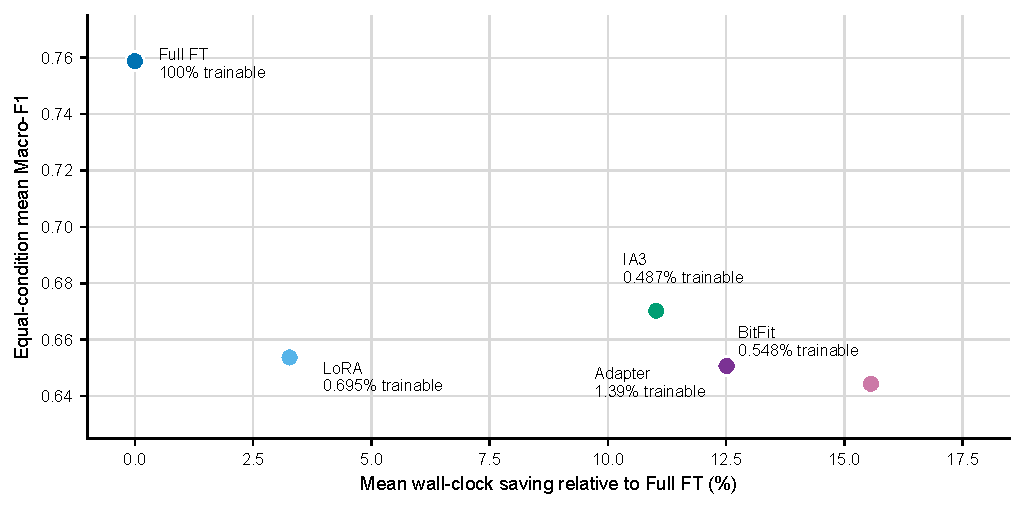
\includegraphics[width=0.88\textwidth]{figures/performance_efficiency_tradeoff.pdf}
\caption{Performance--time trade-off across the original 22 conditions. Labels give mean trainable ratios. The vertical range is expanded to distinguish methods; the precise values are in Table \ref{tab:global}.}
\label{fig:tradeoff}
\end{figure*}

Figure \ref{fig:tradeoff} makes the divergence visible: the methods that save the most time and parameters do not attain the Full FT mean. Parameter ratio is not a proxy for wall-clock time because the frozen backbone still performs forward/backward operations and PEFT modules add implementation overhead.

\subsection{Task-Level Inference and Robustness}

For Macro-F1, the 13-task Friedman result is $Q(4)=24.80$, $p=5.52\times10^{-5}$, $W=0.477$; Iman--Davenport $F(4,48)=10.94$, $p=2.19\times10^{-6}$. Mean ranks are Full FT 1.385, Adapter 2.538, LoRA 3.154, IA3 3.769, and BitFit 4.154. Table \ref{tab:pairwise} reproduces the Full FT comparisons using the preserved generator. Under the fixed policy, every PEFT method is lower after Holm adjustment, but the differences are heterogeneous and contain local wins.

\begin{table*}[!t]
\caption{Task-level PEFT minus Full FT comparisons ($n=13$). CI is a 50,000-resample percentile interval over task blocks; $p_H$ is the exact Wilcoxon value after Holm adjustment; $r_{rb}$ is matched rank-biserial correlation.}
\label{tab:pairwise}
\centering
\footnotesize
\setlength{\tabcolsep}{3.3pt}
\begin{tabular}{lccccccc}
\toprule
Method & Mean $\Delta$ [95\% CI] & Median & HL & $W$ & $p_H$ & $r_{rb}$ & Win/loss \\
\midrule
LoRA & $-0.0906$ [$-0.1952,-0.0118$] & $-0.0209$ & $-0.0210$ & 10 & 0.0242 & $-0.780$ & 1/12 \\
Adapter & $-0.0924$ [$-0.2026,-0.0102$] & $-0.0147$ & $-0.0147$ & 5 & 0.0098 & $-0.890$ & 2/11 \\
IA3 & $-0.0787$ [$-0.1551,-0.0185$] & $-0.0309$ & $-0.0407$ & 10 & 0.0242 & $-0.780$ & 1/12 \\
BitFit & $-0.1002$ [$-0.2099,-0.0189$] & $-0.0290$ & $-0.0344$ & 9 & 0.0242 & $-0.802$ & 1/12 \\
\bottomrule
\end{tabular}
\end{table*}

Training time also differs ($Q=48.31$, $p=8.14\times10^{-10}$, $W=0.929$), as does trainable ratio ($Q=52.00$, $p=1.38\times10^{-10}$, $W=1.000$). The original F1-SD test gives $Q=13.23$, $p=0.0102$, $W=0.254$, but it is not interpreted as a reliability ranking because exact-zero collapse fingerprints contaminate that outcome.

Table \ref{tab:sensitivity} separates two concerns. Removing Study 1 preserves all four Holm decisions. Removing the two collapse-affected tasks preserves a global difference among method ranks but leaves only Adapter below Full FT after Holm control. The strict analysis excluding both concerns has the same qualitative pattern. Thus the global rank difference is robust, whereas ``each PEFT method is individually lower'' is collapse-task sensitive.

\begin{table}[!t]
\caption{Complete-block Macro-F1 sensitivity analyses.}
\label{tab:sensitivity}
\centering
\scriptsize
\setlength{\tabcolsep}{2.8pt}
\begin{tabular}{lrrrrl}
\toprule
Analysis & $n$ & $Q$ & $p$ & $W$ & Holm $p<.05$ \\
\midrule
Original definition & 13 & 24.80 & $5.52\!\times\!10^{-5}$ & .477 & All four \\
Exclude Study 1 & 12 & 21.67 & $2.33\!\times\!10^{-4}$ & .451 & All four \\
Exclude collapse tasks & 11 & 22.62 & $1.51\!\times\!10^{-4}$ & .514 & Adapter \\
Exclude both & 10 & 19.12 & $7.44\!\times\!10^{-4}$ & .478 & Adapter \\
\bottomrule
\end{tabular}
\end{table}

\subsection{Task and Backbone Interactions}

Three local mean leaders prevent a universal-selection claim. IA3 leads on TweetEval hate with RoBERTa (0.5727 vs. Full FT 0.4212) and BERTweet (0.5349 vs. 0.5278); Adapter leads on KLUE YNAT (0.8702 vs. 0.8666). Adapter is within 0.02 of Full FT on each Korean task, but the Korean session uses one model, different tasks, more epochs, and different sample sizes. It is not an estimate of a language effect.

Within the nine Study-2 tasks, averaging over methods favors BERTweet on five tasks and RoBERTa on four. Method-level means favor BERTweet for Full FT, Adapter, IA3, and BitFit, but slightly favor RoBERTa for LoRA. Because model pretraining domain and tokenizer differ, this interaction is descriptive; it does not isolate architecture or domain adaptation causally.

\subsection{Exact-Zero Audit}

Four of the 110 method rows have an exact stored F1 SD of zero and jointly match Eq. (\ref{eq:fingerprint}) (Table \ref{tab:zero-sd}). They are consistent with constant-class collapse, but historical seed predictions are unavailable. The conclusion is therefore about aggregate compatibility, not retrospective observation.

\begin{table*}[!t]
\caption{Original exact-zero rows and constant-class fingerprint metrics.}
\label{tab:zero-sd}
\centering
\scriptsize
\setlength{\tabcolsep}{3.5pt}
\begin{tabular}{lllccccc}
\toprule
Task & Model & Method & Accuracy & Macro precision & Macro recall & Mean F1 & Stored SD \\
\midrule
Finance sentiment & RoBERTa & BitFit & 0.5930 & 0.1977 & 0.3333 & 0.2482 & 0 (exact) \\
Finance sentiment & RoBERTa & Adapter & 0.5930 & 0.1977 & 0.3333 & 0.2482 & 0 (exact) \\
Tweet emotion & RoBERTa & BitFit & 0.3927 & 0.0982 & 0.2500 & 0.1410 & 0 (exact) \\
Tweet emotion & BERTweet & LoRA & 0.3927 & 0.0982 & 0.2500 & 0.1410 & 0 (exact) \\
\bottomrule
\end{tabular}
\end{table*}

Counting all tied minima, BitFit is co-lowest in 10 of 22 conditions, while Adapter is also co-lowest in the Finance/RoBERTa tie; there are 23 assignments across 22 conditions. Excluding only the four fingerprinted rows removes that tie and yields BitFit 8, IA3 5, Full FT 3, LoRA 3, and Adapter 3. This sensitivity shows that ``stability winner'' is not well defined without explicit tie and non-degeneracy rules; it does not prove that every unflagged historical row is healthy.

\subsection{Exploratory Pilot and Full-Data Recovery}

The limited-data pilot baselines collapse in all 20 runs across the four targeted conditions. Table \ref{tab:pilot} reports an exploratory six-configuration comparison for Finance/RoBERTa/Adapter. Because the combined configuration began before several single or partial variants, this is not a prospectively ordered ablation. Longer training, weighting, higher rate, and the tested longer-plus-weighted pair remain collapsed in all five seeds. Only the tested combined remedy provides full class coverage in every seed. Two other two-way combinations were not tested, so the pilot does not show that every component is individually necessary.

\begin{table}[!t]
\caption{Finance/RoBERTa/Adapter pilot (1,024 training examples, five seeds).}
\label{tab:pilot}
\centering
\scriptsize
\setlength{\tabcolsep}{3pt}
\begin{tabular}{lccc}
\toprule
Variant & Macro-F1 & Collapse & Full coverage \\
\midrule
Baseline & $0.2482\pm0.0000$ & 5/5 & 0/5 \\
Longer & $0.2482\pm0.0000$ & 5/5 & 0/5 \\
Weighted & $0.2482\pm0.0000$ & 5/5 & 0/5 \\
Longer + weighted & $0.2482\pm0.0000$ & 5/5 & 0/5 \\
Higher rate & $0.2482\pm0.0000$ & 5/5 & 0/5 \\
Combined remedy & $0.8040\pm0.0063$ & 0/5 & 5/5 \\
\bottomrule
\end{tabular}
\end{table}

Table \ref{tab:followup} gives the 40 full-data paired runs. Every one of the 20 same-seed comparisons favors the remedy. Baseline has 17/20 constant and 18/20 near-collapse runs; remedy has 0/20 of either and predicts all classes in 20/20. All paired-$t$ intervals exclude zero, but the exact sign-flip value is 0.0625 for each condition. We therefore report large, directionally consistent paired differences without a conventional $p<.05$ claim.

\begin{table*}[!t]
\caption{Full-data paired follow-up over seeds 42, 52, 62, 72, and 82. CI is paired-$t$; collapse is baseline $\rightarrow$ remedy; time is remedy/baseline on Apple MPS.}
\label{tab:followup}
\centering
\scriptsize
\setlength{\tabcolsep}{3pt}
\begin{tabular}{lllccccc}
\toprule
Task & Model & Method & Baseline F1 & Remedy F1 & $\Delta$ [95\% CI] & Collapse & Time \\
\midrule
Finance & RoBERTa & Adapter & $0.2759\pm.0338$ & $0.8486\pm.0087$ & .5727 [.5239,.6215] & 2/5$\rightarrow$0/5 & 2.34$\times$ \\
Finance & RoBERTa & BitFit & $0.2482\pm.0000$ & $0.8348\pm.0085$ & .5866 [.5760,.5972] & 5/5$\rightarrow$0/5 & 2.32$\times$ \\
Emotion & RoBERTa & BitFit & $0.1410\pm.0000$ & $0.7646\pm.0056$ & .6236 [.6167,.6306] & 5/5$\rightarrow$0/5 & 2.56$\times$ \\
Emotion & BERTweet & LoRA & $0.1410\pm.0000$ & $0.7840\pm.0037$ & .6430 [.6384,.6475] & 5/5$\rightarrow$0/5 & 2.52$\times$ \\
\bottomrule
\end{tabular}
\end{table*}

\begin{figure*}[!t]
\centering
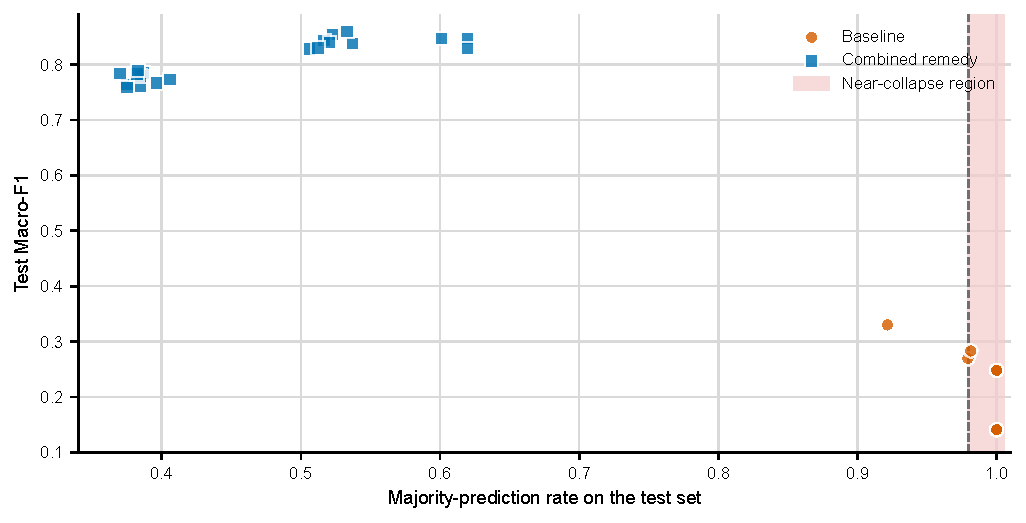
\includegraphics[width=0.88\textwidth]{figures/collapse_diagnostics.pdf}
\caption{Majority-prediction rate and Macro-F1 for the 40 full-data runs. The shaded region begins at the operationally defined 0.98 near-collapse threshold. Remedy runs move to multi-class predictions rather than merely changing a scalar score.}
\label{fig:collapse}
\end{figure*}

Figure \ref{fig:collapse} verifies that the gain accompanies a prediction-distribution change. Finance/Adapter is also a cross-environment warning: its historical aggregate is $0.2482\pm0$, whereas its full-data Apple-MPS baseline is $0.2759\pm0.0338$; the other three baseline aggregates match numerically. The defensible within-follow-up comparison is baseline versus remedy in matched seeds, not historical CUDA versus current MPS or a reranking that substitutes selected remedy cells.


\section{Discussion}

\subsection{No Single Strategy Optimizes Every Criterion}

Full FT is the strongest observed default for predictive performance under the fixed policy, but it is neither fastest nor smallest. BitFit minimizes measured training time, IA3 minimizes trainable state, and Adapter/IA3 lead locally. A useful selection rule should therefore name the objective and constraint rather than declare one global winner.

\begin{table}[!t]
\caption{Evidence-based interpretation guide.}
\label{tab:guide}
\centering
\scriptsize
\setlength{\tabcolsep}{3pt}
\begin{tabularx}{\columnwidth}{lXX}
\toprule
Priority & Observed default & Required check \\
\midrule
Peak F1 & Full FT & Per-task validation and compute budget \\
Fast training & BitFit & Collapse and implementation overhead \\
Small trainable state & IA3 & Task-specific F1 loss \\
Near-Full FT Korean F1 & Adapter & Not a language-effect claim \\
Seed stability & No SD-only winner & Class coverage and prediction distribution \\
\bottomrule
\end{tabularx}
\end{table}

The original broad comparison is a fixed-policy summary retaining all configured condition-level outcomes, including under-trained failures. The follow-up answers a different question: whether a post-selected combined adjustment can recover four fingerprinted cells. Combining them into one leaderboard would give those cells more tuning and epochs than every other cell and would be methodologically unfair.

\subsection{Stability Needs a Non-Degeneracy Gate}

An SD quantifies agreement among seeds; it does not evaluate whether the agreed solution is useful. We recommend a two-stage protocol. First, label constant and operationally defined near-collapse runs using class coverage, majority rate, normalized entropy, and per-class recall. Second, summarize mean, SD, and uncertainty among all runs while reporting the failure rate separately. A performance floor can complement but should not replace output-distribution diagnostics.

The collapse-task sensitivity explains why this is not merely a reporting preference. Removing the two complete task blocks that contain fingerprinted cells leaves a global difference among method ranks but changes three Holm decisions. The pairwise conclusions are therefore sensitive to exclusion of those affected task blocks; this analysis does not isolate the effect of the four cells alone. Collapse auditing belongs before ranking and hypothesis interpretation.

\subsection{Scope of the Recovery Evidence}

No collapse was observed in the 20 tested remedy runs, and Macro-F1 was higher in all 20 same-seed pairs, but the 2.32--2.56-fold time cost is material. The design does not identify whether schedule, learning rate, class weighting, or interaction is the main cause. Finance/Adapter informed the exploratory comparison and is not an independent confirmation; the other three conditions are transfer checks. Five pairs also give coarse exact-test resolution. These results support a targeted recovery recipe, not a universal PEFT optimizer.


\section{Reproducibility and Validity Limits}

The original environment record identifies Python 3.10.19, a PyTorch 2.11 CUDA-development build, CUDA 12.8, NVIDIA RTX 5070 Ti, Transformers 5.9.0, Datasets 4.8.5, and PEFT 0.19.1. Public repository commit 539e3d3 preserves the 110 aggregate rows and 22 winner rows, but not the 550 historical run-level predictions, configurations, checkpoints, or exact optimizer, scheduler, model-revision, and dataset-revision evidence. Consequently, the stored aggregates and downstream calculations can be audited, but the historical executions cannot be replayed bit for bit.

The locally retained full-data follow-up ran on Apple MPS with Python 3.13.7, PyTorch 2.13.0, Transformers 5.9.0, Datasets 4.8.5, PEFT 0.19.1, and five matched seeds. Its 40 runs preserve predictions, metrics, histories, configurations, model commits, and split fingerprints; 60 pilot runs preserve analogous local artifacts, although their per-run device field is unavailable. Metric recomputation from all 100 saved prediction files produced zero discrepancies. Compact metric-level rows for those runs are released, while per-example predictions and other detailed run artifacts remain local. Moreover, the recorded executed \texttt{src/suite.py} hash differs from the current source, and the exact executed snapshot was not preserved; the current source is therefore not claimed to be bit-identical to the executed file.

\textbf{Artifact availability:} the historical aggregate remains traceable to public repository commit \href{https://github.com/LEESY-X/Domain_fine-tuning_experiments/tree/539e3d3}{\underline{539e3d3}}. Versioned reconstruction/re-execution code, configurations, the historical aggregate tables, and compact metric-level records for all 60 pilot and 40 full-data follow-up runs are available in tagged snapshot \href{https://github.com/LEESY-X/Domain_fine-tuning_experiments/tree/ieie-spc-v1.0.0}{\underline{ieie-spc-v1.0.0}}; Appendix A states its scope. Per-example predictions and histories were validated locally but are not public, so their prediction-level check is not independently repeatable from the tag. Raw dataset text, checkpoints, and caches are not redistributed. No archive DOI has been assigned.

\textbf{Validity limits:} Study 1 lacks a historical group-wise split manifest; sensitivity excluding it is therefore reported. The 13 task blocks share datasets, code, and backbones, so their exchangeability is an analysis assumption rather than established independence. The collapse fingerprint is analytical because original predictions are absent. Follow-up hardware differs from the historical environment, the four conditions were selected after observing exact zeros, and each paired condition has only five seeds. Near-collapse at 0.98 is an operational threshold. Macro-F1, parameter ratio, and \texttt{trainer.train()} time do not measure calibration, inference latency, memory, energy, or distribution shift. The model/task/epoch confounding prevents a causal language comparison. The convenience benchmark is not a random sample of domains, so task-level $p$-values do not establish population-wide generalization.


\section{Conclusion}

The integrated evidence resolves the apparent contradiction in the original paper. Full FT delivers the strongest broad fixed-policy performance, while BitFit and IA3 lead different efficiency objectives and PEFT methods win selected tasks. At the same time, four apparently perfect zero-SD results are consistent with constant-class collapse, and removing their tasks weakens several pairwise claims. A targeted combined remedy yields higher Macro-F1 in all 20 tested seed pairs and no collapse in the 20 remedy runs, but costs more time and does not reach an exact two-sided $p<.05$ with five pairs. Fine-tuning strategy selection is therefore multi-objective, task conditional, and collapse aware: report performance, time, trainable state, and prediction-distribution failures separately.

\appendixt{Code and Compact Evidence Snapshot}

The versioned repository is available as \href{https://github.com/LEESY-X/Domain_fine-tuning_experiments/tree/ieie-spc-v1.0.0}{\underline{release v1.0.0}}. It contains the maintained code and configurations, the 110-row historical aggregate and 22-row winner table, compact run-level metrics and collapse diagnostics for the 60 pilot and 40 full-data follow-up runs, environment records, a run-coverage manifest, validation notes, and SHA-256 checksums. It excludes dataset text and caches, checkpoints, per-example predictions, trainer histories, events, and per-run JSON files. The compact records support regeneration of reported summaries and paired statistics, but not independent per-example metric recomputation or bit-identical replay of the unavailable executed source snapshot.


\section*{Acknowledgment}

OpenAI Codex was used for manuscript restructuring, language editing, reproducible table/figure generation, and consistency checks. The authors remain responsible for the study design, source data, statistical interpretation, and final manuscript.


\begin{reference}

\bibitem{1} J. Devlin, M.-W. Chang, K. Lee, and K. Toutanova, ``BERT: Pre-training of deep bidirectional transformers for language understanding,'' in \textit{Proc. NAACL-HLT}, pp. 4171--4186, 2019. \href{https://doi.org/10.18653/v1/N19-1423}{\underline{Article}}

\bibitem{2} Y. Liu et al., ``RoBERTa: A robustly optimized BERT pretraining approach,'' \textit{arXiv:1907.11692}, 2019. \href{https://doi.org/10.48550/arXiv.1907.11692}{\underline{Article}}

\bibitem{3} D. Q. Nguyen, T. Vu, and A. T. Nguyen, ``BERTweet: A pre-trained language model for English Tweets,'' in \textit{Proc. EMNLP System Demonstrations}, pp. 9--14, 2020. \href{https://doi.org/10.18653/v1/2020.emnlp-demos.2}{\underline{Article}}

\bibitem{4} S. Park et al., ``KLUE: Korean Language Understanding Evaluation,'' in \textit{Advances in Neural Information Processing Systems: Datasets and Benchmarks}, 2021. \href{https://arxiv.org/abs/2105.09680}{\underline{Article}}

\bibitem{5} N. Houlsby et al., ``Parameter-efficient transfer learning for NLP,'' in \textit{Proc. 36th Int. Conf. Machine Learning}, vol. 97, pp. 2790--2799, 2019. \href{https://proceedings.mlr.press/v97/houlsby19a.html}{\underline{Article}}

\bibitem{6} E. J. Hu et al., ``LoRA: Low-rank adaptation of large language models,'' in \textit{Proc. Int. Conf. Learning Representations}, 2022. \href{https://openreview.net/forum?id=nZeVKeeFYf9}{\underline{Article}}

\bibitem{7} H. Liu et al., ``Few-shot parameter-efficient fine-tuning is better and cheaper than in-context learning,'' in \textit{Advances in Neural Information Processing Systems}, vol. 35, 2022. \href{https://openreview.net/forum?id=rBCvMG-JsPd}{\underline{Article}}

\bibitem{8} E. Ben Zaken, Y. Goldberg, and S. Ravfogel, ``BitFit: Simple parameter-efficient fine-tuning for transformer-based masked language-models,'' in \textit{Proc. 60th Annual Meeting of the ACL}, pp. 1--9, 2022. \href{https://doi.org/10.18653/v1/2022.acl-short.1}{\underline{Article}}

\bibitem{9} N. Reimers and I. Gurevych, ``Reporting score distributions makes a difference: Performance study of LSTM-networks for sequence tagging,'' in \textit{Proc. EMNLP}, pp. 338--348, 2017. \href{https://doi.org/10.18653/v1/D17-1035}{\underline{Article}}

\bibitem{10} J. Dodge et al., ``Fine-tuning pretrained language models: Weight initializations, data orders, and early stopping,'' \textit{arXiv:2002.06305}, 2020. \href{https://doi.org/10.48550/arXiv.2002.06305}{\underline{Article}}

\bibitem{11} F. Barbieri, J. Camacho-Collados, L. Espinosa-Anke, and L. Neves, ``TweetEval: Unified benchmark and comparative evaluation for tweet classification,'' in \textit{Findings of EMNLP}, pp. 1644--1650, 2020. \href{https://doi.org/10.18653/v1/2020.findings-emnlp.148}{\underline{Article}}

\bibitem{12} P. Malo, A. Sinha, P. Takala, P. Korhonen, and J. Wallenius, ``Good debt or bad debt: Detecting semantic orientations in economic texts,'' \textit{J. Association for Information Science and Technology}, vol. 65, no. 4, pp. 782--796, 2014. \href{https://doi.org/10.1002/asi.23062}{\underline{Article}}

\bibitem{13} A. L. Maas et al., ``Learning word vectors for sentiment analysis,'' in \textit{Proc. 49th Annual Meeting of the ACL}, pp. 142--150, 2011. \href{https://aclanthology.org/P11-1015/}{\underline{Article}}

\bibitem{14} P. Keung, Y. Lu, G. Szarvas, and N. A. Smith, ``The multilingual Amazon Reviews Corpus,'' in \textit{Proc. EMNLP}, pp. 4563--4568, 2020. \href{https://doi.org/10.18653/v1/2020.emnlp-main.369}{\underline{Article}}

\bibitem{15} X. Zhang, J. Zhao, and Y. LeCun, ``Character-level convolutional networks for text classification,'' in \textit{Advances in Neural Information Processing Systems}, vol. 28, 2015. \href{https://arxiv.org/abs/1509.01626}{\underline{Article}}

\bibitem{16} J. Lee et al., ``K-MHaS: A multi-label hate speech detection dataset in Korean online news comment,'' in \textit{Proc. 29th Int. Conf. Computational Linguistics}, pp. 3530--3538, 2022. \href{https://aclanthology.org/2022.coling-1.311/}{\underline{Article}}

\bibitem{17} M. Mosbach, M. Andriushchenko, and D. Klakow, ``On the stability of fine-tuning BERT: Misconceptions, explanations, and strong baselines,'' in \textit{Proc. Int. Conf. Learning Representations}, 2021. \href{https://openreview.net/forum?id=nzpLWnVAyah}{\underline{Article}}

\bibitem{18} Y. Du and D. Nguyen, ``Measuring the instability of fine-tuning,'' in \textit{Proc. 61st Annual Meeting of the ACL}, pp. 6209--6230, 2023. \href{https://doi.org/10.18653/v1/2023.acl-long.342}{\underline{Article}}

\bibitem{19} N. T. Bui, G. Savova, and L. Wang, ``Assessing the macro and micro effects of random seeds on fine-tuning large language models,'' in \textit{Proc. IJCNLP-AACL Short Papers}, pp. 41--46, 2025. \href{https://doi.org/10.18653/v1/2025.ijcnlp-short.3}{\underline{Article}}

\bibitem{20} Y. Mao et al., ``UniPELT: A unified framework for parameter-efficient language model tuning,'' in \textit{Proc. 60th Annual Meeting of the ACL}, pp. 6253--6264, 2022. \href{https://doi.org/10.18653/v1/2022.acl-long.433}{\underline{Article}}

\bibitem{21} V. Lialin, V. Deshpande, X. Yao, and A. Rumshisky, ``Scaling down to scale up: A guide to parameter-efficient fine-tuning,'' \textit{arXiv:2303.15647}, 2023. \href{https://arxiv.org/abs/2303.15647}{\underline{Article}}

\bibitem{22} P. S. Sachdeva et al., ``The Measuring Hate Speech Corpus: Leveraging Rasch measurement theory for data perspectivism,'' in \textit{Proc. 1st Workshop on Perspectivist Approaches to NLP}, pp. 83--94, 2022. \href{https://aclanthology.org/2022.nlperspectives-1.11/}{\underline{Article}}

\bibitem{23} Y. Hong and J. Kim, ``Evaluating fine-tuning performance variations of BERT models using the GLUE benchmark,'' \textit{The Korea Journal of BigData}, vol. 10, no. 2, pp. 95--109, 2025. \href{https://doi.org/10.36498/kbigdt.2025.10.2.95}{\underline{Article}}

\bibitem{24} J. Dem\v{s}ar, ``Statistical comparisons of classifiers over multiple data sets,'' \textit{J. Machine Learning Research}, vol. 7, pp. 1--30, 2006. \href{https://jmlr.org/papers/v7/demsar06a.html}{\underline{Article}}

\bibitem{25} S. Holm, ``A simple sequentially rejective multiple test procedure,'' \textit{Scandinavian J. Statistics}, vol. 6, no. 2, pp. 65--70, 1979. \href{https://www.jstor.org/stable/4615733}{\underline{Article}}

\bibitem{26} e9t, ``Naver Sentiment Movie Corpus v1.0,'' GitHub repository. \href{https://github.com/e9t/nsmc}{\underline{Repository}} (accessed Jul. 14, 2026).

\bibitem{27} UC Berkeley D-Lab, ``Measuring Hate Speech,'' Hugging Face dataset card, 2024. \href{https://doi.org/10.57967/hf/2710}{\underline{Dataset card}}

\end{reference}


\biography{}{Yuseok Hong}{Yuseok Hong is affiliated with the Major in Big Data Convergence at Sangmyung University, Seoul, Republic of Korea. His research interests include natural language processing, parameter-efficient learning, and reproducible evaluation of machine-learning systems.}

\biography{}{Seonyeok Lee}{Seonyeok Lee is affiliated with the Major in Big Data Convergence at Sangmyung University, Seoul, Republic of Korea. His research interests include natural language processing and empirical evaluation of language models.}

\biography{}{Sooyong Lee}{Sooyong Lee is affiliated with the Major in Big Data Convergence at Sangmyung University, Seoul, Republic of Korea. His research interests include machine learning, text classification, and reproducible experimentation.}

\vfill
\relax

\endofpaper

\end{document}
